\documentclass{ctexart}
\usepackage{Note}
\begin{document}
\setcounter{FormalCounter}{0}
\section{线性回归}
\subsection{单变量线性拟合}
\subsubsection{简单多项式拟合与误差函数}
实际的数据集通常没有明显的规律,或者内含的规律被随机分布的噪声所隐藏.对于回归问题,最简单的方式就是通过多项式进行拟合.\\
\indent 假定训练集为包含$N$组数据的集合$\left\{\left(x_1,y_1\right),\cdots,\left(x_N,y_N\right)\right\}$,其中各$x_i$为自变量,各$y_i$为真实值.我们考虑形式如下的多项式函数以预测自变量$x$对应的值(其中$\hat{y}$表示$y$的预测值):
\[\hat{y}=f(x;\vec{w})=w_0+w_1x+\cdots+w_Mx^M=\sum_{j=0}^{M}w_jx^j\]
\begin{definition}[拟合多项式的阶数]
    上述拟合多项式中最高次项的次数$M$被称作拟合多项式的\tbf{阶数}.
\end{definition}
\begin{definition}[权重矢量]
    权重矢量$\vec{w}$是拟合多项式的参数构成的矢量.例如,上述多项式的权重矢量即为
    \[\vec{w}=\left(w_0,w_1,\cdots,w_M\right)\]
\end{definition}
给定多项式的阶数,我们能写出很多可能的拟合多项式.为了得出与数据集相差最小的多项式,我们需要定义\tbf{误差函数}以衡量预测值与实际值之间的差距.
\begin{definition}[误差函数]
    \tbf{误差函数(Error Function)}(或称\tbf{代价函数(Cost Function)})是衡量模型预测值$\hat{y}$与实际值$y$之间的差距的函数.\\
    机器学习中常用的误差函数为\tbf{平方和误差函数(Sum-of-Square Error Function)},即\tbf{二乘\footnotemark 误差函数}:
    \[E(\vec{w})=\dfrac12\sum_{i=1}^{N}\left(\hat{y_i}-y_i\right)^2=\dfrac12\sum_{i=1}^{N}\left(f(x_i;\vec{w})-y_i\right)^2\]
\end{definition}\footnotetext{这里的二乘即平方.另外,函数前的系数$1/2$是为了方便计算而采取的取法.}
\begin{definition}[最小二乘多项式拟合]
    使用二乘误差函数的多项式拟合称作最小二乘多项式拟合.
\end{definition}
容易看出这与统计学中最小二乘法的关系.显然,误差函数越小,模型给出的预测值$\hat{y}$整体而言与目标值$y$越接近.
\subsubsection{拟合多项式的求法:以线性回归为例}
线性拟合是最简单的多项式拟合的方法.使用一次函数模型
\[f(x)=ax+b\]
进行拟合,那么权重矢量$\vec{w}=(a,b)$.我们有如下结论:
\begin{theorem}[简单线性回归的参数]
    假定训练集为包含$N$组数据的集合$\left\{\left(x_1,y_1\right),\cdots,\left(x_N,y_N\right)\right\}$,采取模型$f(x)=ax+b$进行拟合,误差函数为二乘误差函数,那么得到的结果应为
    \[a=\dfrac{\overline{xy}-\bar{x}\bar{y}}{\overline{x^2}-{\bar{x}}^2}\ \ \ \ \ \ b=\dfrac{\overline{x^2}\bar{y}-\bar{x}\cdot\overline{xy}}{\overline{x^2}-{\bar{x}}^2}\]
    其中$\bar{*}$代表基于训练集数据得到的平均值.
\end{theorem}
\begin{proof}
    误差函数$E(\vec{w})$的自变量为$\vec{w}$,具有两个独立的参数$a,b$.为了让$E(\vec{w})$最小,我们不妨对$a,b$分别求偏导,并令偏导数为$0$.
    \[\left\{\begin{array}{l}
        \displaystyle\dfrac{\p E}{\p a}=\sum_{i=1}^{N}\left(ax_i+b-y_i\right)x_i=0\\
        \displaystyle\dfrac{\p E}{\p b}=\sum_{i=1}^{N}\left(ax_i+b-y_i\right)=0
    \end{array}\right.\]
    整理可得
    \[\left\{\begin{array}{l}
        \displaystyle a\sum_{i=1}^{N}x_i^2+b\sum_{i=1}^{N}x_i-\sum_{i=1}^{N}x_iy_i=0\\
        \displaystyle a\sum_{i=1}^{N}x_i+bN-\sum_{i=1}^{N}y_i=0
    \end{array}\right.\]
    解这个方程组即可得到定理中的结论.
\end{proof}
对于一般的简单多项式拟合问题,都可以用求偏导数的方法进行求解.
\subsubsection{过拟合与正则化}
我们用一组简单的数据说明过拟合这一现象.考虑由$\sin(2\pi x)$附加正态分布的噪声所构成的数据,由下面的程序给出:
\begin{lstlisting}
import numpy as np
x = np.arange(-0.5, 0.5, 0.1)  # 生成 x 值,步长 0.1
y = np.sin(2 * np.pi * x)
y_noisy = y + np.random.normal(loc=0, scale=np.sqrt(0.3), size=x.shape)  # 添加方差为 0.3 的正态分布噪声
\end{lstlisting}
现在我们把拟合的结果呈现如下:
\begin{figure}[H]
    \centering
    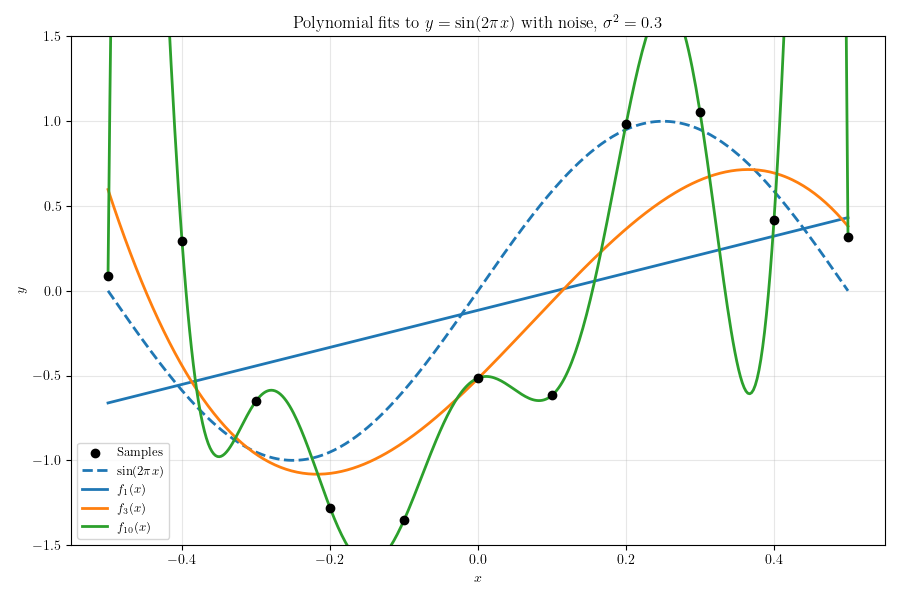
\includegraphics[width=0.8\textwidth]{figure/overfitting.png}
    \caption{不同阶数的多项式拟合}
\end{figure}
如图所示,我们用不同阶数的多项式对数据进行拟合.可以看到,线性拟合的效果并不好,而阶数为$3$的多项式拟合则相对而言比较接近实际值.随着阶数的增加,拟合效果变得越来越好.然而,当阶数过高时(例如这里采取的阶数为$10$),拟合曲线开始出现剧烈的振荡,并且在数据点之间的区域偏离了真实函数.可以想见,在一般的测试集上,高阶多项式的拟合效果会变得很差.
\begin{definition}[过拟合]
    当模型在训练数据上表现良好,但在未见过的数据上表现较差时,我们称模型发生了\tbf{过拟合(Overfitting)}现象.
\end{definition}
\indent 过拟合的原因在于,复杂的函数具有更强的表达能力,能够更好地拟合训练数据(上面的$f_{10}$对每个数据点都没有偏差),但同时也会受到数据中的噪声影响,导致模型在训练数据之外的表现变差.\\
\indent 除了在测试集中较差的表现之外,过拟合的另一个特征是模型的参数值变得非常大.这和曲线的明显振荡是对应的.\\
\indent 解决过拟合问题的一个简单办法是增加测试集的规模,或减小模型的复杂度.另一种常用的方法是\tbf{正则化(Regularization)}.
\begin{definition}[正则化]
    \tbf{正则化(Regularization)}是通过在误差函数中加入对模型复杂度的惩罚项,以防止模型过拟合的一种技术.
\end{definition}
例如,我们可以使用如下的正则化误差函数:
\[\tilde{E}(\vec{w})=\dfrac12\sum_{i=1}^{N}\left(\hat{y_i}-y_i\right)^2+\dfrac{\lambda}{2}\left|\left|\vec{w}\right|\right|^2\]
代替原来的误差函数进行拟合.其中$\lambda$为正则化参数,控制正则化项的权重.如果$\lambda=0$,那么没有惩罚;$\lambda$越大,惩罚越强,此时模型倾向于用更小的参数进行拟合.$\lambda$极大时,$\vec{w}$的各参数接近$0$,是一条接近横轴的平坦的线.通过调整$\lambda$,我们可以在拟合训练数据和符合测试数据之间找到一个平衡点.
\subsubsection{维度灾难}
当输入数据$\vec{x}$的分量较多时,我们称其为高维数据.例如,一张$28\times 28$的灰度图像可以看作是一个$784$维的向量.\\
\indent 高维数据的一个重要问题是\tbf{维度灾难(Curse of Dimensionality)}.
\begin{definition}[维度灾难]
    维度灾难是指随着数据维度的增加,数据量需求呈指数级增长,从而导致计算和存储的巨大开销,以及模型难以捕捉数据的真实分布等问题.
\end{definition}
前面所举的例子中的$\vec{x}$是一维的,这是很容易用多项式拟合的.但是,如果类似的方法用到高维数据上就有很大的问题了.对于一张分辨率为$640\times480$的图像,每个像素采用RGB表示,那么一张图像就可以看作是一个$640\times480\times3=921600$维的向量.如果仍然采用多项式拟合,那么需要的各阶参数数量为
\[N_0=1\ \ \ \ \ N_1=921600\ \ \ \ \ N_2=C_{921600}^2=424354112000\ \ \ \ \ N_3=C_{921600}^3=1.303\times10^{17}\cdots\]
很难找到足够的训练数据来拟合这些参数.\\
\indent 简单而言,维度的增加对数据量的要求是指数增长的,而数据量本身却是有限的.这就导致了维度灾难.此外,高维空间中的点往往是稀疏分布的;高维空间的球绝大部分分布于球面附近,这些反直觉的性质使得模型难以捕捉数据的真实分布.\\
\indent 例如,采用监督学习的方式让程序分辨猫和狗,很有可能程序采用与猫和狗无关的特征来进行分类,例如图像的亮度,特定像素点的数目等,从而导致模型在测试集上表现不佳.
\subsection{从概率论的角度看待线性回归}
\subsubsection{正态分布与最小二乘法}
通常,我们假定观测值$y$可以写成下面的形式:
\[y=g(x;\vec{w})+\epsilon\]
其中$g(x;\vec{w})$是一个确定的函数,显示了数据的内在规律; $\epsilon$为噪声.大部分时候,我们都假设噪声满足均值为$0$,方差为$\sigma$的正态分布.
\begin{definition}[正态分布]
    随机变量$X$服从均值为$\mu$,方差为$\sigma^2$的\tbf{正态分布(Normal Distribution)}(或称\tbf{高斯分布(Gaussian Distribution)}),如果它的概率密度函数为
    \[p(X=x)=\dfrac{1}{\sqrt{2\pi\sigma^2}}\exp\left(-\dfrac{(x-\mu)^2}{2\sigma^2}\right)\equiv\mathcal{N}\left(x|\mu,\sigma^2\right)\]
\end{definition}
这样,对于给定的自变量$x_i$和观测值$t_i$,其概率为
\[P\left(t_i|x_i\right)=P\left(\ep=t_i-g\left(x_i;\vec{w}\right)\right)=\mathcal{N}\left(t_i-g\left(x_i;\vec{w}\right)|0,\sigma^2\right)=\mathcal{N}\left(t_i|g\left(x_i;\vec{w}\right),\sigma^2\right)\]
假定各组数据是相互独立的,并且各处的噪声满足同一分布(即方差$\sigma^2$在各处相同)那么整个数据集的概率函数为
\[P\left(\{t_i\}| \{x_i\}\right)=\prod_{i=1}^{N}P\left(t_i|x_i\right)=\prod_{i=1}^{N}\mathcal{N}\left(t_i|g\left(x_i;\vec{w}\right),\sigma^2\right)\]
在不引起混淆的情况下,数据集也可以用粗体字母表示,例如$\mbf{t}=\{t_i\},\mbf{x}=\{x_i\}$.另外按机器学习领域的惯例,记$\beta=\dfrac{1}{\sigma^2}$,于是上述概率函数可以写成
\[P\left(\mbf{t}|\mbf{x},\vec{w};\beta\right)=\prod_{i=1}^{N}\mathcal{N}\left(t_i|g\left(x_i,\vec{w}\right),\beta^{-1}\right)\]
在训练过程中,我们只知道训练集$\mbf{x}$与$\mbf{t}$,不知道参数$\vec{w}$与$\beta$.直观而言\footnote{我们将在后面详细讨论贝叶斯公式以完善对这种直观的严谨叙述.},我们希望选择一组参数$\vec{w},\beta$,使得在这组参数下,观测到训练集的概率最大.这就是\tbf{极大似然估计(Maximum Likelihood Estimation)}的思想.\\
\indent 对于连乘函数的最值估计,通常先取对数后再考虑.于是上述概率函数取对数后得到
\[\ln P\left(\mbf{t}|\mbf{x},\vec{w},\beta\right)=\sum_{i=1}^{N}\ln\mathcal{N}\left(t_i|g\left(x_i;\vec{w}\right),\beta^{-1}\right)=-\dfrac{\beta}{2}\sum_{i=1}^{N}\left(g\left(x_i;\vec{w}\right)-t_i\right)^2+\dfrac{N}{2}\ln\beta-\dfrac{N}{2}\ln(2\pi)\]
与训练集有关的项即前面的求和项.回顾二乘误差函数的定义:
\[E(\vec{w})=\dfrac12\sum_{i=1}^{N}\left(g(x_i;\vec{w})-t_i\right)^2\]
仍然采用偏导等于$\mbf{0}$的办法,即
\[\dfrac{\p}{\p \vec{w}}\ln P\left(\mbf{t}|\mbf{x},\vec{w},\beta\right)=-\beta\dfrac{\p E(\vec{w})}{\p \vec{w}}=\mbf{0}\]
我们就可以得到与最小二乘法相同的结果,即拟合函数为
\[f\left(x;\vec{w}_{\text{ML}}\right)=g\left(x;\vec{w}_{\text{ML}}\right)\]
这里的$\vec{w}_{\text{ML}}$表示极大似然估计得到的参数,与前面推导中的一般权重矢量$\vec{w}$不同.\\
\indent 这说明在噪声服从正态分布的假设下,最小二乘法实际上是极大似然估计的一种实现方式.另外,我们还可以根据前面的推导求出噪声的表达形式:
\[\dfrac{1}{\beta}=\sigma^2=
\dfrac{1}{N}\sum_{i=1}^{N}\left(f\left(x_i;\vec{w}_{\text{ML}}\right)-t_i\right)^2\]
\subsection{Bayes定理}
\begin{theorem}[Bayes定理]
    设$A,B$为两个事件,且$P(B)>0$,那么
    \[P(A|B)=\dfrac{P(B|A)P(A)}{P(B)}\]
    其中$P(A)$与$P(B)$分别为事件$A$与事件$B$的概率, 又称为\tbf{先验概率}; $P(A|B)$与$P(B|A)$分别为在事件$B$发生的条件下事件$A$发生的概率,又称为\tbf{后验概率}与\tbf{似然函数}.
\end{theorem}
\begin{proof}
    由条件概率的定义,我们有
    \[P(A|B)=\dfrac{P(A\cap B)}{P(B)}\ \ \ \ \ \ P(B|A)=\dfrac{P(A\cap B)}{P(A)}\]
    整理可得Bayes定理.
\end{proof}
\begin{problem}
    如果你的邻居购买了$n$张彩票,并且其中有$m$张是中奖的,请估计你购买一张彩票中奖的概率.\\
    \textit{注意:在你没有购买彩票之前,你对中奖概率一无所知,因此只能假定中奖概率是均匀分布的,即它是$[0,1]$上等概率取的一个数.}
\end{problem}
\begin{solution}
    由于本题涉及的中奖概率是连续变量,因此下面的概率均为概率密度函数.设中奖概率为$x$,那么买$n$张彩票而中$m$张的概率密度函数为
    \[P(m,n|x)=C_n^mx^m(1-x)^{n-m}\]
    根据Bayes定理,我们有
    \[P(x|m,n)=\dfrac{P(m,n|x)P(x)}{P(m,n)}\]
    而
    \[P(m,n)=\int_{0}^{1}P(m,n|x)P(x)\di x\]
    由于$x$在$[0,1]$上均匀分布,因此$P(x)=1$.于是
    \[P(x|m,n)=\dfrac{P(m,n|x)}{\displaystyle\int_0^1P(m,n|x)\di x}=\dfrac{C_n^mx^m(1-x)^{n-m}}{\displaystyle\int_0^1C_n^mx^m(1-x)^{n-m}\di x}=\dfrac{x^m(1-x)^{n-m}}{\displaystyle\int_0^1x^m(1-x)^{n-m}\di x}
    =\dfrac{x^m(1-x)^{n-m}}{\text{B}(m+1,n-m+1)}\]
    这里的$\text{B}$表示Beta函数.对于连续变量$x$而言,我们最好用期望来表示$x$的估计值.因此
    \[\hat{x}=\int_0^1xP(x|m,n)\di x=\dfrac{\displaystyle\int_0^1x^{m+1}(1-x)^{n-m}\di x}{\text{B}(m+1,n-m+1)}=\dfrac{\text{B}(m+2,n-m+1)}{\text{B}(m+1,n-m+1)}=\dfrac{m+1}{n+2}\]
    也即,我们估计买彩票中奖的概率为$\dfrac{m+1}{n+2}$.这是符合直觉的,因为当$m=0$时,我们也不应估计中奖概率为$0$;同理,当$m=n$时,我们也不应估计中奖概率为$1$.买的越多,估计的结果就越接近$m/n$,也就越准确.
\end{solution}
现在,我们把目光重新放回机器学习上.把Bayes定理写成如下形式:
\[p(\vec{w}|\mathcal{D})=\dfrac{p(\mathcal{D}|\vec{w})p(\vec{w})}{p(\mathcal{D})}\]
这里的$\mathcal{D}$表示训练集,而$\vec{w}$表示模型参数.
\begin{definition}[先验分布,后验分布和似然函数]
    在上述Bayes定理中,$p(\vec{w})$称为\tbf{先验分布(Prior Distribution)},表示在给定训练集之前对参数$\vec{w}$的认识; $p(\vec{w}|\mathcal{D})$称为\tbf{后验分布(Posterior Distribution)},表示在给定训练集之后对参数$\vec{w}$的认识; $p(\mathcal{D}|\vec{w})$称为\tbf{似然函数(Likelihood Function)},表示在给定参数$\vec{w}$的条件下观测到训练集的概率.
\end{definition}
公式中的$p(\mathcal{D})$是一个归一化常数,与参数$\vec{w}$无关,通常就不去特意考虑.因此,为了获取后验分布,我们只需要计算似然函数与先验分布的乘积.\\
\indent 最简单的处理方法,就是假定先验分布是均匀分布,即对所有可能的参数$\vec{w}$都一视同仁.此时,后验分布与似然函数成正比,如果我们取概率最大的$\vec{w}$作为拟合问题的解,这时的似然函数就最大.这就是\tbf{极大似然估计}.
\begin{definition}[极大似然估计]
    通过选择使似然函数$p\left(\mathcal{D}|\vec{w}\right)$最大的参数$\vec{w}$来拟合数据的方式,称为\tbf{极大似然估计(Maximum Likelihood Estimation)}.
\end{definition}
\indent 有时,我们已经对先验分布$p(\vec{w})$有一定的估计.综合考虑$p(\mathcal{D}|\vec{w})$与$p(\vec{w})$的乘积,选择使得后验分布最大的参数$\vec{w}$作为拟合问题的解,这就是\tbf{极大后验估计}.
\begin{definition}[极大后验估计]
    通过选择使后验分布$p\left(\vec{w}|\mathcal{D}\right)$最大的参数$\vec{w}$来拟合数据的方式,称为\tbf{极大后验估计(Maximum A Posteriori Estimation)}.
\end{definition}
下面给出了极大后验估计的一个例子.
\begin{problem}
    在过拟合一节中,我们讲到参数越大越容易过拟合的情形,即认为$||\vec{w}||$越大越不可能,这是与$\mathcal{D}$无关的先验知识.\\
    现在,假定$\vec{w}$的范数满足正态分布:
    \[p\left(\vec{w}|\alpha\right)=\mathcal{N}\left(||\vec{w}||\left|0,\frac{1}{\alpha}\right.\right)=\left(\dfrac{\alpha}{2\pi}\right)^{\frac{M+1}{2}}\exp\left(-\dfrac{\alpha||\vec{w}||^2}{2}\right)\]
    求极大后验估计的结果.
\end{problem}
\begin{solution}
    由Bayes定理,我们有
    \[p(\vec{w}|\mathcal{D})=\dfrac{p(\mathcal{D}|\vec{w})p(\vec{w}|\alpha)}{p(\mathcal{D})}\]
    由于$p(\mathcal{D})$与$\vec{w}$无关,因此我们只需考虑分子部分.取对数后得到
    \[\ln p(\vec{w}|\mathcal{D})=\ln p(\mathcal{D}|\vec{w})+\ln p(\vec{w}|\alpha)+\text{const}\]
    假定似然函数仍然为
    \[P\left(\mathcal{D}|\vec{w},\beta\right)=\prod_{i=1}^{N}\mathcal{N}\left(t_i|g\left(x_i,\vec{w}\right),\beta^{-1}\right)\]
    忽略与$\vec{w}$无关的项可得
    \[\ln p(\vec{w}|\mathcal{D})=-\dfrac{\beta}{2}\sum_{i=1}^{N}\left(g\left(x_i;\vec{w}\right)-t_i\right)^2-\dfrac{\alpha}{2}||\vec{w}||^2+\text{const}\]
    这与前述正则化误差函数
    \[\tilde{E}(\vec{w})=\dfrac12\sum_{i=1}^{N}\left(g(x_i;\vec{w})-t_i\right)^2+\dfrac{\lambda}{2}||\vec{w}||^2\]
    在形式上一致.事实上,如果取$\lambda=\dfrac{\alpha}{\beta}$,那么极大后验估计与正则化误差函数的结果是一样的.\\
    \indent 同样不难想到,对$p(\vec{w})$的不同估计对应不同的正则化误差函数.
\end{solution}
然而,前面所述的方法都是频率学派所用的方法\footnote{尽管我们使用了Bayes定理,但仍然是在做点估计,}.频率学派认为应该根据随机事件重复的频率来考察概率,而概率是完全先验的,不会因为数据而改变.例如,无论如何抛一枚质地均匀的硬币,它的正反面朝上的概率都是$\dfrac12$,即使已经抛出了连续$100$次正面.在机器学习中,这意味着模型的参数是固定的,而数据是依照一定的规律随机分布的.\\
\indent 贝叶斯学派与频率学派观点相左.他们认为数据才是固定的,模型的参数则是随机的,并且服从某种分布.例如,抛一枚硬币,如果已经抛出了连续$100$次正面,那么我们就有理由怀疑这枚硬币不是均匀的,而是正面朝上的概率更大.在机器学习中,这意味着数据是固定的,我们只能对模型的参数有一个最初的估计,这一估计会随着数据的增加而改变,最终得到比较准确的结论.\\
\indent 贝叶斯学派的观点与极大后验估计的思想是一致的.然而,贝叶斯学派并不满足于只求出一个最优的参数$\vec{w}$,而是希望得到参数的整个分布.
\end{document}